\section{SCADA}
\frame{
	\ifdebug
	\frametitle{Outline\hfill{\color{red} \emph{A}}}
	\else
	\frametitle{Outline}
	\fi
	\tableofcontents[currentsection]
	}

\subsection*{Intro Scada}

\frame{
	\ifdebug
	\frametitle{Introducción SCADA\hfill{\color{red} \emph{A}}}
	\else
	\frametitle{Introducción SCADA}
	\fi
	\textbf{PLC:} realiza automáticamente las tareas de control 
	    pre-programado sobre un proceso.
	   
	\textbf{Problema:} no presenta una manera sencilla de
	\begin{columns}
	 \begin{column}{0.3\textwidth}
	 \begin{itemize}
	   \item Supervisar
	   \item Adaptar
	 \end{itemize}
	 \end{column}
	 \begin{column}{0.7\textwidth}
	  El comportamiento del sistema.
	 \end{column}
	\end{columns}
	
	\begin{columns}
	\begin{column}{0.5\textwidth}
	  \textbf{Solución}:\\
	  \textbf{SCADA}: Supervisory Control And Data Adquisition
	 \end{column}
	 \begin{column}{0.5\textwidth}
	  \begin{figure}[ht!]
	    \centering
	    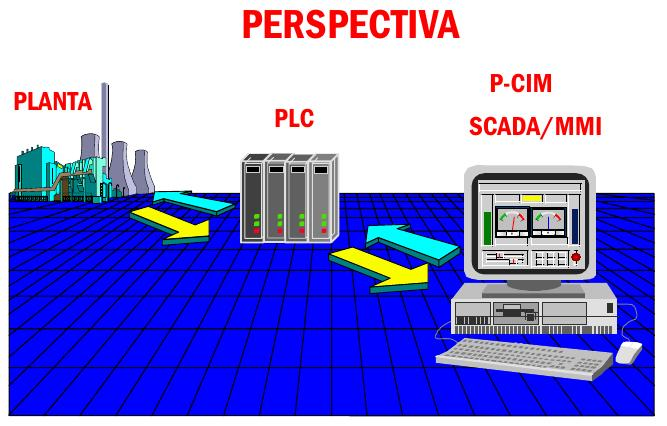
\includegraphics[width=\textwidth]
	    {../Informe/Cap5-SCADA/images/perspectiva.jpeg}
	\end{figure}
	 \end{column}
	\end{columns}
}

\subsection*{Estructura PCIM}
\frame{
	\ifdebug
	\frametitle{P-CIM - AFCON\hfill{\color{red} \emph{A}}}
	\else
	\frametitle{P-CIM - AFCON}
	\fi
	\begin{columns}[T]
	  \begin{column}{0.3\textwidth}
	    \begin{figure}
	      \centering
	      
\includegraphics[width=\textwidth]
	      {Sections/5-Scada/images/afcon.pdf}
	    \end{figure}
	      \footnotesize
	      Entorno de desarrollo y ejecución de aplicaciones SCADA.
	  \end{column}	 
	  \begin{column}{0.6\textwidth}
	    Su estructura se compone de 3 capas:
	    \begin{itemize}
	     \item Comunicación
	     \item Procesamiento de Datos
	     \item Aplicaciones
	    \end{itemize}
	  \begin{figure}[ht!]
	  \centering
		  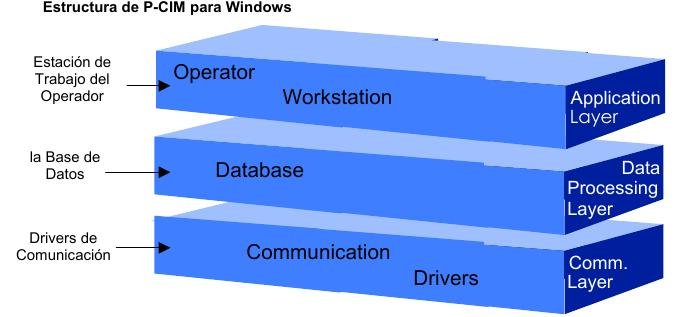
\includegraphics[width=\textwidth]
		  {../Informe/Cap5-SCADA/images/estructura.jpeg}
	  \end{figure}
	  \end{column}

	\end{columns}
}

\frame{
	\ifdebug
	\frametitle{Capa de Comunicación\hfill{\color{red} \emph{A}}}
	\else
	\frametitle{Capa de Comunicación}
	\fi
	\begin{columns}
	 \begin{column}{0.4\textwidth}
	    \textbf{Modbus}:\begin{itemize}
	                       \item Protocolo de Facto en la industria
	                       \item Gran disponibilidad
	                       \item Libre desde 2004
	                      \end{itemize}

	  \end{column}
	  \begin{column}{0.6\textwidth}
	    \begin{figure}
	     
\includegraphics[width=\textwidth]
	      {Sections/5-Scada/images/modbus_logo.png}
	    \end{figure}
	  \end{column}
	\end{columns}

	\vspace{1cm}
	Para la implementación de la capa de comunicación en P-CIM:
	\begin{columns}[T]
	  \begin{column}{0.3\textwidth}
	    \textbf{Instalación}
	    \begin{figure}
	     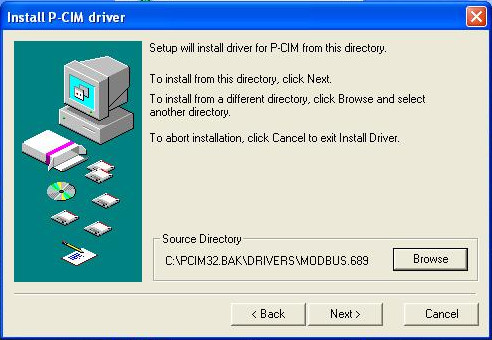
\includegraphics[width=\textwidth]
	      {../Informe/Cap5-SCADA/images/installDriver.jpeg}
	    \end{figure}
	  \end{column}
	  \begin{column}{0.3\textwidth}
	   \textbf{Configuración}
	   \begin{figure}
	    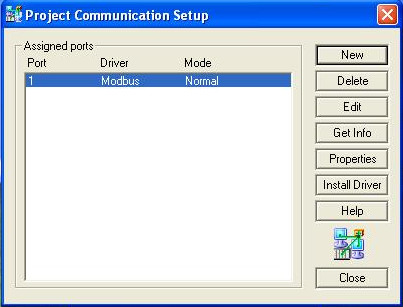
\includegraphics[width=\textwidth]
	      {../Informe/Cap5-SCADA/images/commSetup.jpeg}
	   \end{figure}
	  \end{column}
	  \begin{column}{0.3\textwidth}
	   \textbf{Obtener Información}
	  \begin{figure}
	   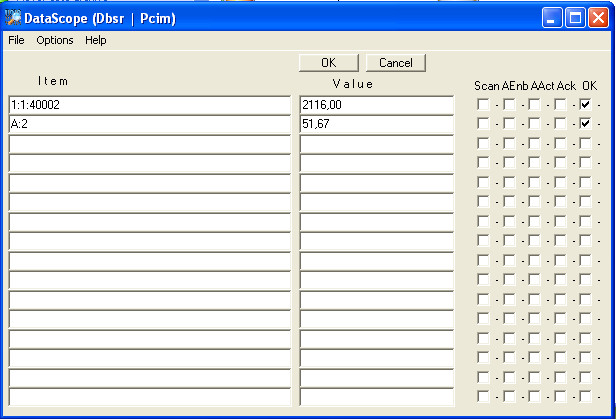
\includegraphics[width=0.8\textwidth]
	    {../Informe/Cap5-SCADA/images/dataScope.jpeg}
	  \end{figure}
	 \end{column}
	\end{columns}
}

\frame{
	\ifdebug
	\frametitle{Capa de Procesamiento\hfill{\color{red} \emph{A}}}
	\else
	\frametitle{Capa de Procesamiento}
	\fi
	\textbf{Base de Datos}: recupera, almacena y procesa la
información de tiempo real que recibe desde la capa de comunicación
	\begin{figure*}[!ht]
  \centering 
  \resizebox{\textwidth}{!}{
  
  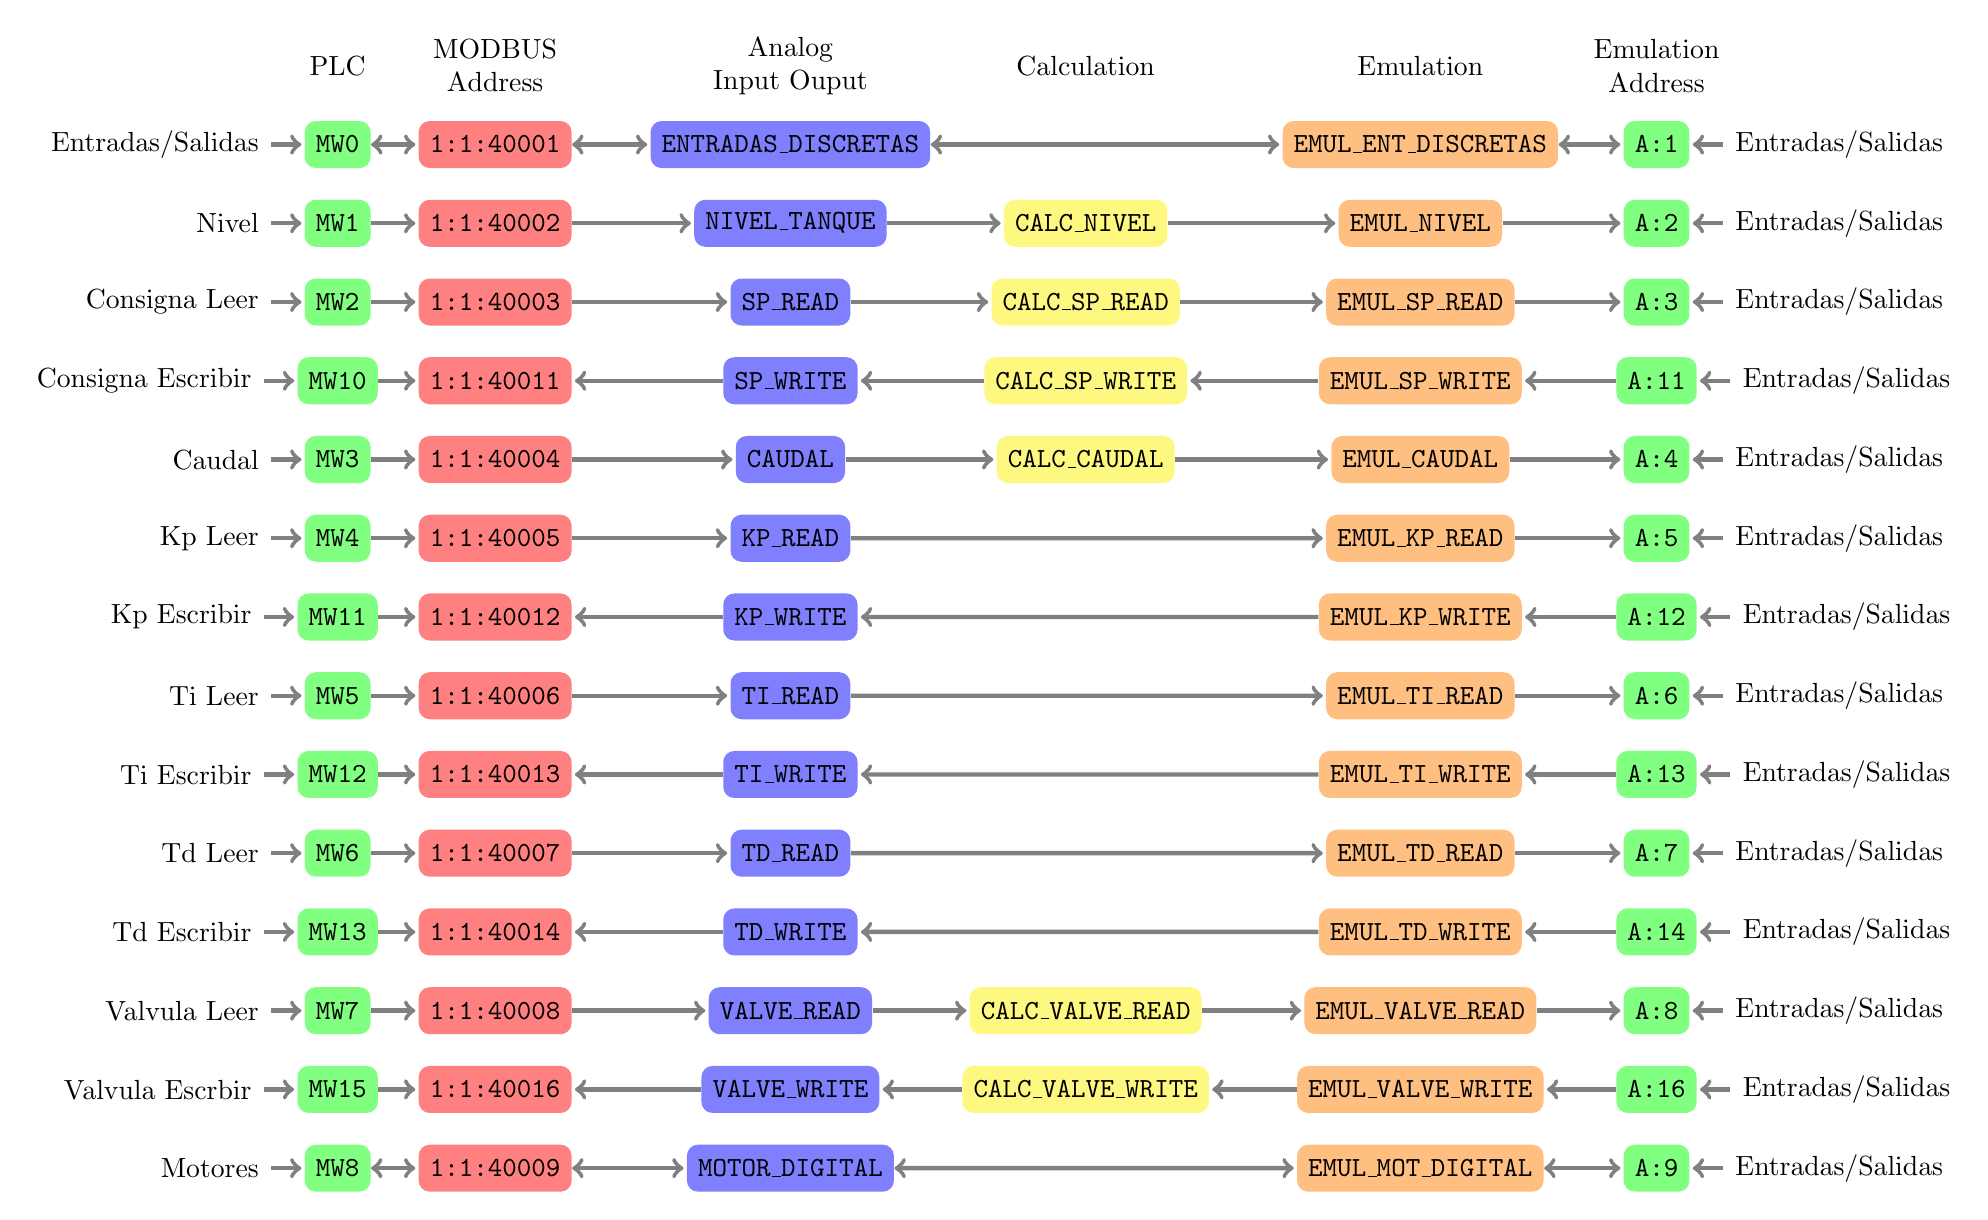
\begin{tikzpicture}[shorten >=1pt,->,draw=black!50]
    \tikzstyle{every pin edge}=[<-,shorten <=1pt, ultra thick]
    \tikzstyle{neuron}=[rectangle,fill=black!25,minimum size=17pt,inner 
sep=4pt, rounded corners]
    \tikzstyle{annot} = [text width=7em, text centered]

    \tikzstyle{plc neuron}=[neuron, fill=green!50];
    \tikzstyle{modbus neuron}=[neuron, fill=red!50, node 
    distance=0.4*5cm];
    \tikzstyle{aio neuron}=[neuron, fill=blue!50, node 
    distance=0.75*5cm];
    \tikzstyle{calc neuron}=[neuron, fill=yellow!50, node 
    distance=0.75*5cm];
    \tikzstyle{emul neuron}=[neuron, fill=orange!50, node 
    distance=0.85*5cm];
    \tikzstyle{emula neuron}=[neuron, fill=green!50, node 
    distance=0.6*5cm];

    % Draw the plc layer nodes
     \node[plc neuron, pin=left:Entradas/Salidas] (mw0) at (0,0) 
{\texttt{MW0}};
     \node[plc neuron, pin=left:Nivel] (mw1) at (0,-1) 
{\texttt{MW1}};
     \node[plc neuron, pin=left: Consigna Leer] (mw2) at (0,-2) 
{\texttt{MW2}};
     \node[plc neuron, pin=left: Consigna Escribir] (mw10) at (0,-3) 
{\texttt{MW10}};
     \node[plc neuron, pin=left: Caudal] (mw3) at (0,-4) 
{\texttt{MW3}};
      \node[plc neuron, pin=left: Kp Leer] (mw4) at (0,-5) 
 {\texttt{MW4}};
      \node[plc neuron, pin=left: Kp Escribir] (mw11) at (0,-6) 
 {\texttt{MW11}};
      \node[plc neuron, pin=left: Ti Leer] (mw5) at (0,-7) 
 {\texttt{MW5}};
      \node[plc neuron, pin=left: Ti Escribir] (mw12) at (0,-8) 
 {\texttt{MW12}};
      \node[plc neuron, pin=left: Td Leer] (mw6) at (0,-9) 
 {\texttt{MW6}};
      \node[plc neuron, pin=left: Td Escribir] (mw13) at (0,-10) 
 {\texttt{MW13}};
      \node[plc neuron, pin=left: Valvula Leer] (mw7) at (0,-11) 
 {\texttt{MW7}};
      \node[plc neuron, pin=left: Valvula Escrbir] (mw15) at (0,-12) 
 {\texttt{MW15}};
      \node[plc neuron, pin=left: Motores] (mw8) at (0,-13) 
 {\texttt{MW8}};

    %Draw Modbus layer nodes
    \node[modbus neuron, right of=mw0] (40001)  {\texttt{1:1:40001}};
    \node[modbus neuron, right of=mw1] (40002)  {\texttt{1:1:40002}};
    \node[modbus neuron, right of=mw2] (40003)  {\texttt{1:1:40003}};
    \node[modbus neuron, right of=mw3] (40004)  {\texttt{1:1:40004}};
    \node[modbus neuron, right of=mw4] (40005)  {\texttt{1:1:40005}};
    \node[modbus neuron, right of=mw5] (40006)  {\texttt{1:1:40006}};
    \node[modbus neuron, right of=mw6] (40007)  {\texttt{1:1:40007}};
    \node[modbus neuron, right of=mw7] (40008)  {\texttt{1:1:40008}};
    \node[modbus neuron, right of=mw8] (40009)  {\texttt{1:1:40009}};
    \node[modbus neuron, right of=mw10] (40011)  {\texttt{1:1:40011}};
    \node[modbus neuron, right of=mw11] (40012)  {\texttt{1:1:40012}};
    \node[modbus neuron, right of=mw12] (40013)  {\texttt{1:1:40013}};
    \node[modbus neuron, right of=mw13] (40014)  {\texttt{1:1:40014}};
    \node[modbus neuron, right of=mw15] (40016)  {\texttt{1:1:40016}};
     
    %Draw Analog Input Output layer nodes
    \node[aio neuron, right of=40001] (io)  {\texttt{ENTRADAS\_DISCRETAS}};
    \node[aio neuron, right of=40002] (niv)  {\texttt{NIVEL\_TANQUE}};
    \node[aio neuron, right of=40003] (spr)  {\texttt{SP\_READ}};
    \node[aio neuron, right of=40004] (caudal)  {\texttt{CAUDAL}};
    \node[aio neuron, right of=40005] (kpr)  {\texttt{KP\_READ}};
    \node[aio neuron, right of=40006] (tir)  {\texttt{TI\_READ}};
    \node[aio neuron, right of=40007] (tdr)  {\texttt{TD\_READ}};
    \node[aio neuron, right of=40008] (vr)  {\texttt{VALVE\_READ}};
    \node[aio neuron, right of=40009] (md)  {\texttt{MOTOR\_DIGITAL}};
    \node[aio neuron, right of=40011] (spw)  {\texttt{SP\_WRITE}};
    \node[aio neuron, right of=40012] (kpw)  {\texttt{KP\_WRITE}};
    \node[aio neuron, right of=40013] (tiw)  {\texttt{TI\_WRITE}};
    \node[aio neuron, right of=40014] (tdw) {\texttt{TD\_WRITE}};
    \node[aio neuron, right of=40016] (vw)  {\texttt{VALVE\_WRITE}};

    %Draw Calculation
    \node[calc neuron, right of=niv] (cniv) {\texttt{CALC\_NIVEL}};
    \node[calc neuron, right of=spr] (cspr) {\texttt{CALC\_SP\_READ}};
    \node[calc neuron, right of=spw] (cspw) {\texttt{CALC\_SP\_WRITE}};
    \node[calc neuron, right of=caudal] (ccaudal) {\texttt{CALC\_CAUDAL}};
    \node[calc neuron, right of=vr] (cvr) {\texttt{CALC\_VALVE\_READ}};
    \node[calc neuron, right of=vw] (cvw) {\texttt{CALC\_VALVE\_WRITE}};
    
    %Draw ResultCalculation
    \node[emul neuron, right of=cniv] (eniv) {\texttt{EMUL\_NIVEL}};
    \node[emul neuron, right of=cspr] (espr) {\texttt{EMUL\_SP\_READ}};
    \node[emul neuron, right of=cspw] (espw) {\texttt{EMUL\_SP\_WRITE}};
    \node[emul neuron, right of=ccaudal] (ecaudal) {\texttt{EMUL\_CAUDAL}};
    \node[emul neuron, right of=cvr] (evr) {\texttt{EMUL\_VALVE\_READ}};
    \node[emul neuron, right of=cvw] (evw) {\texttt{EMUL\_VALVE\_WRITE}};
    
    %Draw Emulation
    \node[emul neuron] (eio) at (2.75*5cm,0 cm) 
{\texttt{EMUL\_ENT\_DISCRETAS}};
    \node[emul neuron] (ekpr) at (2.75*5cm,-5 cm) 
{\texttt{EMUL\_KP\_READ}};
    \node[emul neuron] (etir) at (2.75*5cm,-7 cm) 
{\texttt{EMUL\_TI\_READ}};
    \node[emul neuron] (etdr) at (2.75*5cm,-9 cm) 
{\texttt{EMUL\_TD\_READ}};
    \node[emul neuron] (emd) at (2.75*5cm,-13 cm) 
{\texttt{EMUL\_MOT\_DIGITAL}};
    \node[emul neuron] (ekpw) at (2.75*5cm,-6 
cm){\texttt{EMUL\_KP\_WRITE}};
    \node[emul neuron] (etiw) at (2.75*5cm,-8 cm) 
{\texttt{EMUL\_TI\_WRITE}};
    \node[emul neuron] (etdw) at (2.75*5cm,-10 cm) 
{\texttt{EMUL\_TD\_WRITE}};

    %Draw internal variables
   \node[emula neuron, pin=right:Entradas/Salidas,right of=eio] (a1) 
  {\texttt{A:1}};
  \node[emula neuron, pin=right:Entradas/Salidas,right of=eniv] (a2) 
  {\texttt{A:2}};
  \node[emula neuron, pin=right:Entradas/Salidas,right of=espr] (a3) 
  {\texttt{A:3}};
  \node[emula neuron, pin=right:Entradas/Salidas,right of=espw] (a11) 
  {\texttt{A:11}};
  \node[emula neuron, pin=right:Entradas/Salidas,right of=ecaudal] (a4) 
  {\texttt{A:4}};
  \node[emula neuron, pin=right:Entradas/Salidas,right of=ekpr] (a5) 
  {\texttt{A:5}};
  \node[emula neuron, pin=right:Entradas/Salidas,right of=ekpw] (a12) 
  {\texttt{A:12}};
  \node[emula neuron, pin=right:Entradas/Salidas,right of=etir] (a6) 
  {\texttt{A:6}};
  \node[emula neuron, pin=right:Entradas/Salidas,right of=etiw] (a13) 
  {\texttt{A:13}};
  \node[emula neuron, pin=right:Entradas/Salidas,right of=etdr] (a7) 
  {\texttt{A:7}};
  \node[emula neuron, pin=right:Entradas/Salidas,right of=etdw] (a14) 
  {\texttt{A:14}};
  \node[emula neuron, pin=right:Entradas/Salidas,right of=evr] (a8) 
  {\texttt{A:8}};
  \node[emula neuron, pin=right:Entradas/Salidas,right of=evw] (a16) 
  {\texttt{A:16}};
  \node[emula neuron, pin=right:Entradas/Salidas,right of=emd] (a9) 
  {\texttt{A:9}};

   
  % Connect every node 
  %PLC -> MODBUS
  \path (mw0) edge[<->,ultra thick] (40001); 
  \path (mw1) edge[ultra thick] (40002); 
  \path (mw2) edge[ultra thick] (40003);
  \path (mw3) edge[ultra thick] (40004); 
  \path (mw4) edge[ultra thick] (40005); 
  \path (mw5) edge[ultra thick] (40006); 
  \path (mw6) edge[ultra thick] (40007); 
  \path (mw7) edge[ultra thick] (40008); 
  \path (mw8) edge[<->,ultra thick] (40009);
  \path (mw10) edge[ultra thick] (40011); 
  \path (mw11) edge[ultra thick] (40012); 
  \path (mw12) edge[ultra thick] (40013);
  \path (mw13) edge[ultra thick] (40014); 
  \path (mw15) edge[ultra thick] (40016); 

  %MODBUS -> Analog IO
  \path (40001) edge[<->,ultra thick] (io); 
  \path (40002) edge[ultra thick] (niv); 
  \path (40003) edge[ultra thick] (spr);
  \path (40004) edge[ultra thick] (caudal);
  \path (40005) edge[ultra thick] (kpr);
  \path (40006) edge[ultra thick] (tir);
  \path (40007) edge[ultra thick] (tdr); 
  \path (40008) edge[ultra thick] (vr);
  \path (40009) edge[<->,ultra thick] (md); 
  \path (spw) edge[ultra thick] (40011); 
  \path (kpw) edge[ultra thick] (40012);
  \path (tiw) edge[ultra thick] (40013); 
  \path (tdw) edge[ultra thick] (40014);
  \path (vw) edge[ultra thick] (40016); 

  %Analog -> Calc
  \path (niv) edge[ultra thick] (cniv);
  \path (spr) edge[ultra thick] (cspr);
  \path (cspw) edge[ultra thick] (spw);
  \path (caudal) edge[ultra thick] (ccaudal);
  \path (vr) edge[ultra thick] (cvr);
  \path (cvw) edge[ultra thick] (vw);

  %Calc -> Emulation
  \path (cniv) edge[ultra thick] (eniv);
  \path (cspr) edge[ultra thick] (espr);
  \path (espw) edge[ultra thick] (cspw);
  \path (ccaudal) edge[ultra thick] (ecaudal);
  \path (cvr) edge[ultra thick] (evr);
  \path (evw) edge[ultra thick] (cvw); 
  
  %Analog IO -> Emulation
  \path (io) edge[<->,ultra thick] (eio);
  \path (kpr) edge[ultra thick] (ekpr);
  \path (ekpw) edge[ultra thick] (kpw);
  \path (tir) edge[ultra thick] (etir);
  \path (etiw) edge[ultra thick] (tiw);
  \path (tdr) edge[ultra thick] (etdr);
  \path (etdw) edge[ultra thick] (tdw);
  \path (md) edge[<->,ultra thick] (emd);

  %Emulation -> Address
  \path (eio) edge[<->,ultra thick] (a1);
  \path (eniv) edge[ultra thick] (a2);
  \path (espr) edge[ultra thick] (a3);
  \path  (a11) edge[ultra thick] (espw);
  \path (ecaudal) edge[ultra thick] (a4);
  \path (ekpr) edge[ultra thick] (a5);
  \path  (a12) edge[ultra thick] (ekpw);
  \path (etir) edge[ultra thick] (a6);
  \path  (a13) edge[ultra thick] (etiw);
  \path (etdr) edge[ultra thick] (a7);
  \path (a14) edge[ultra thick] (etdw);
  \path (evr) edge[ultra thick] (a8);
  \path (a16) edge[ultra thick] (evw);
  \path (emd) edge[<->,ultra thick] (a9);
  

 
  % Annotate the layers
  \node[annot,above of=mw0, node distance=1cm] (plc) {PLC};
  \node[annot,above of=40001, node distance=1cm] (modbus) {MODBUS Address};
  \node[annot,above of=io, node distance=1cm] (aio) {Analog Input Ouput};
  \node[annot,right of=aio, node distance=0.75*5cm] (calc) {Calculation};
  \node[annot,above of=eio, node distance=1cm] (emul) {Emulation};
  \node[annot,above of=a1, node distance=1cm] (emula) {Emulation Address};

\end{tikzpicture}
  }
    \caption{Conexion de bloques de la Base de Datos}
    \label{fig:bloqDB}
\end{figure*}
}

\frame{
	\ifdebug
	\frametitle{Capa de Aplicación\hfill{\color{red} \emph{A}}}
	\else
	\frametitle{Capa de Aplicación}
	\fi
	Última capa del SCADA, antes de que la información llegue al operario

	\vspace{.5cm}
	\begin{columns}[t]
	\begin{column}{0.35\textwidth}
	\textbf{Requerimientos:}
	\begin{itemize}
	\item Reducir la complejidad de la supervisión del sistema
	\item Actuar de manera remota sobre la planta y su controlador
	\end{itemize}
	\end{column}
	\begin{column}{0.65\textwidth}
	\textbf{Diseño:}
	\begin{figure}[!ht]
	\centering
	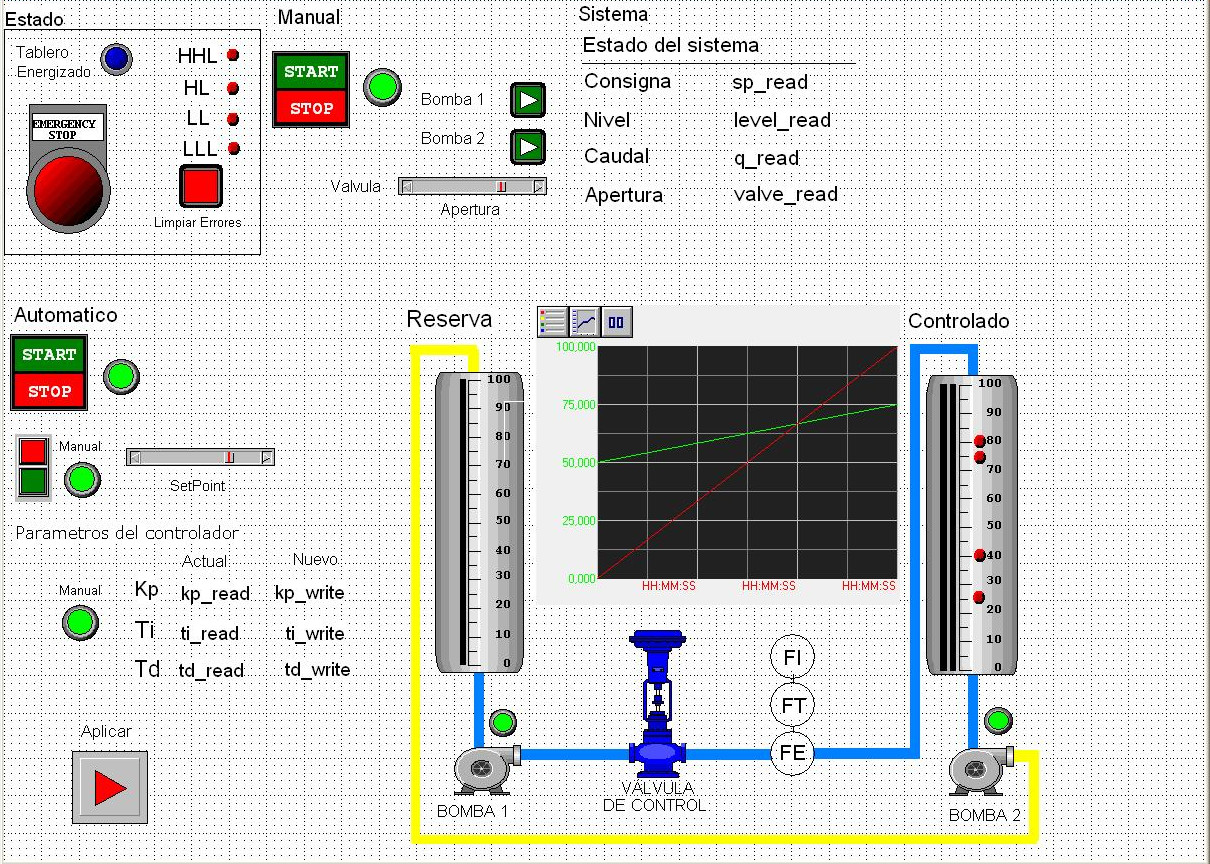
\includegraphics[width=\textwidth]
	{../Informe/Cap5-SCADA/images/hmiScada.jpeg}
	\end{figure}

	\end{column}

	\end{columns}
}

% \frame{
% 	\frametitle{Slide de gracia}
% 	\begin{columns}
% 		\begin{column}{0.4\textwidth}
% 			\begin{enumerate}
% 				\item Una
% 				\begin{itemize}
% 					\item \textbf{Larga}
% 					\item larga
% 				\end{itemize}
% 				\item Lista
% 			\end{enumerate}
% 
% 			\begin{align*}
% 				\mathrm{una} \,e( \textbf{cuacion})
% 			\end{align*}
% 		\end{column}
% 
% 		\begin{column}{0.6\textwidth}
% 			\begin{center}
% 				\missingfigure[figwidth=4.5cm]{}
% 			\end{center}
% 
% 			\begin{center}
% 				\footnotesize
% 				\textbf{\textit{Cita bibliográfica}}
% 
% 				[Escrita por alguien \textit{et al.} 2008]
% 			\end{center}
% 		\end{column}
% 
% 	\end{columns}
% }